%%%%%%%%%%%%%%%%%%%%%%%%%%%%%%%%%%%%%%%%%%%%%%%%
%% Compile the master file!
%% 		Slides: Antonio Machicao y Priemer
%% 		Course: GK Linguistik
%%%%%%%%%%%%%%%%%%%%%%%%%%%%%%%%%%%%%%%%%%%%%%%%

%%%%%%%%%%%%%%%%%%%%%%%%%%%%%%%%%%%%%%%%%%%%%%%%%%%%
%%%             Metadata                        
%%%%%%%%%%%%%%%%%%%%%%%%%%%%%%%%%%%%%%%%%%%%%%%%%%%%      

\title{Grundkurs Linguistik}

\subtitle{Syntax I: Einführung \& Terminologie}

\author[A. Machicao y Priemer]{
	{\small Antonio Machicao y Priemer}
	\\
	{\footnotesize \url{http://www.linguistik.hu-berlin.de/staff/amyp}}
	%	\\
	%	\href{mailto:mapriema@hu-berlin.de}{mapriema@hu-berlin.de}}
}

\institute{Institut für deutsche Sprache und Linguistik}


% bitte lassen, sonst kann man nicht sehen, von wann die PDF-Datei ist.
%\date{ }

%\publishers{\textbf{6. linguistischer Methodenworkshop \\ Humboldt-Universität zu Berlin}}


%%%%%%%%%%%%%%%%%%%%%%%%%%%%%%%%%%%%%%%%%%%%%%%%%%%%
%%%             Preamble's End                  
%%%%%%%%%%%%%%%%%%%%%%%%%%%%%%%%%%%%%%%%%%%%%%%%%%%%      


%%%%%%%%%%%%%%%%%%%%%%%%%      
\huberlintitlepage[22pt]
\iftoggle{toc}{
\frame{
%\begin{multicols}{2}
	\frametitle{Inhaltsverzeichnis}\tableofcontents
	%[pausesections]
%\end{multicols}
	}
	}


%%%%%%%%%%%%%%%%%%%%%%%%%%%%%%%%%%
%%%%%%%%%%%%%%%%%%%%%%%%%%%%%%%%%%
%%%%%LITERATURE:

%% Allgemein
\nocite{Glueck&Roedel16a}
\nocite{Grewendorf&Co91a}
\nocite{Luedeling2009a}
\nocite{Meibauer&Co07a}
\nocite{Repp&Co15a}

%% Morphologie
%\nocite{Eisenberg04}

%% Syntax
\nocite{Adger04a}
\nocite{Brandt&Co06a} 
\nocite{Fries&MyP16b} % Akzeptabilität
\nocite{Fries16a} % Grammatikalität
\nocite{Fries&MyP16d} % Kompetenz vs Performanz
%\nocite{Fries&MyP16c} % GG
%\nocite{Fries&MyP16a} % X-Bar-Theorie
%\nocite{Fries16e} % Satztyp
%\nocite{Fries16d} % Satzmodus 
\nocite{Grewendorf&Co91a} 
\nocite{MyP18a} % Konstituententest
\nocite{MyP18b} % Kopf
\nocite{MyP18c} % Phrase
\nocite{MyP18g} %Entscheidungsfragesatz
\nocite{MyP18i} %Ergänzungsfragesatz
%\nocite{MuellerS13f} 
%\nocite{MuellerS15b}
%\nocite{Stechow&Sternefeld88a}
%\nocite{Sternefeld06a}
%\nocite{Sternefeld06b}

%%%%%%%%%%%%%%%%%%%%%%%%%%%%%%%%%%%
%%%%%%%%%%%%%%%%%%%%%%%%%%%%%%%%%%


%%%%%%%%%%%%%%%%%%%%%%%%%%%%%%%%%%%%
%%%%%%%%%%%%%%%%%%%%%%%%%%%%%%%%%%%
%\section{Kontakt}
%%\frame{
%%\frametitle{~}
%%	\tableofcontents[currentsection]
%%}
%
%
%%%%%%%%%%%%%%%%%%%%%%%%%%%%%%%%%%%
%\begin{frame}
%\frametitle{Kontakt}
%
%
%\scalebox{0.90}{
%
%\begin{tabular}{ll}
%\textbf{Dozent:} & Antonio Machicao y Priemer \\ 
%			     & \textipa{[ma.\t{tS}i."ka.o.""Pi."pKi:.m5]}\\
%			     &	\\
%\textbf{E-Mail:} & \href{mailto:mapriema@hu-berlin.de}{mapriema@hu-berlin.de} \\ 
%\textbf{Webseite:} & \url{http://www.linguistik.hu-berlin.de/staff/amyp} \\ 
%					& \\
%\textbf{Büro:} & Dorotheenstraße 24, Raum: 3.305 \\
%\textbf{Telefonnummer:} & +49(30)-2093-9702 \\
%				& \\
%\textbf{Sprechstunde:} & Freitags 15--16 (Anmeldung per E-Mail erforderlich!) \\ 
% & \\
%\textbf{Sekretariat:} & Anina Klein \\
%\textbf{E-Mail:} & \href{mailto:Anina.Klein@cms.hu-berlin.de}{Anina.Klein@cms.hu-berlin.de} \\
%\textbf{Büro:} & Dorotheenstraße 24, Raum: 3.306 \\
%\textbf{Telefonnummer:} & +49(30)-2093-9639 \\
%\end{tabular} 
%
%}
%\end{frame}
%
%
%%%%%%%%%%%%%%%%%%%%%%%%%%%%%%%%%%%%
%%%%%%%%%%%%%%%%%%%%%%%%%%%%%%%%%%%
%\section{Formalia}
%%\frame{
%%\frametitle{~}
%%	\tableofcontents[currentsection]
%%}
%
%
%%%%%%%%%%%%%%%%%%%%%%%%%%%%%%%%%%%
%\begin{frame}\frametitle{Formalia}
%
%\begin{itemize}
%	\item \textbf{Leistungserbringung}
%	
%	\begin{itemize}
%		\item Regelmäßige und aktive Teilnahme
%		\item[+]
%		\item Im ersten Teil (CM):\\
%		Probeklausur (zu 50\% bestehen)\\
%		ODER\\
%		2 Hausaufgabenlösungen vorstellen
%		\item[+]
%		\item Im zweiten Teil (AMyP):\\
%		Bestehen (mind. 50\%) einer größeren Hausaufgabe (Syntax / Semantik)
%		\item[+]
%		\item Modulabschlussprüfung (GK Linguistik + UE Deutsche Grammatik)
%		\end{itemize}
%\end{itemize}
%
%\end{frame}
%
%
%%%%%%%%%%%%%%%%%%%%%%%%%%%%%%%%%%%
%\begin{frame}\frametitle{Formalia}
%
%\begin{itemize}
%	\item Was wird noch erwartet?
%	
%	\begin{itemize}
%		\item Die angegebene Literatur bitte lesen! 
%		\item[]
%		\item Fragen und Diskussionen!
%		\item[]
%		\item Kein FB, Twitter, Tumblr, Youtube, WhatsApp, Netflix \dots
%		\item[]
%		\item Wenn Sie früher gehen müssen, sagen Sie mir bitte zu Beginn der Stunde Bescheid, und nehmen Sie bitte Platz in der Nähe der Tür.
%
%	\end{itemize}
%\end{itemize}
%
%\end{frame}

%%%%%%%%%%%%%%%%%%%%%%%%%%%%%%%%%%

\begin{frame}
	\frametitle{Begleitlektüre}
	
	\begin{itemize}
		\item \textbf{obligatorisch:}
			\begin{itemize}
				\item[] AM S.~55--69
			\end{itemize}
	\end{itemize}
\end{frame}

%%%%%%%%%%%%%%%%%%%%%%%%%%%%%%%%%%%%
\section{Syntax I}
%%%%%%%%%%%%%%%%%%%%%%%%%%%%%%%%%%%%

\subsection{Was ist Syntax?}

\iftoggle{sectoc}{
	\frame{
		%\begin{multicols}{2}
		\frametitle{~}
		\tableofcontents[currentsubsection,subsubsectionstyle=hide]
		%\end{multicols}
	}
}


%%%%%%%%%%%%%%%%%%%%%%%%%%%%%%%%%%
\begin{frame}

\begin{figure}
	\centering
\scalebox{.8}{\begin{forest} MyP edges,
	[S
		[NP [N$'$
			[AdjP [Adj$'$ [\zerobar{Adj} [\alertred{Colorless}] ] ]]
			[N$'$
				[AdjP [Adj$'$ [\zerobar{Adj} [\alertred{green}] ] ] ]
				[N$'$ [\zerobar{N} [\alertred{ideas}] ] ]
			]
		]]
		[VP [V$'$
			[V$'$ [\zerobar{V} [\alertred{sleep}] ] ]
			[AdvP [Adv$'$ [\zerobar{Adv} [\alertred{furiously}] ] ] ]
		] ]
	]
\end{forest}}
\end{figure}

\end{frame}


%%%%%%%%%%%%%%%%%%%%%%%%%%%%%%%%%%
\begin{frame}
\frametitle{Was ist Syntax?}

\begin{itemize}
	\item Syntax $=$ Zusammenstellung (griech.\ \MyPobj{sýn}: \gq{zusammen}, \MyPobj{tàxis}: \gq{Ordnung})
	\item[]
	\item \textbf{Zusammenstellung} und \textbf{Struktur} von Phrasen (und Sätzen) aus kleineren Elementen (Wörtern)
\end{itemize}

\nocite{Roedel16a}

\end{frame}

%%%%%%%%%%%%%%%%%%%%%%%%%%%%%%%%%%%%%%%%%%%%%%%%%%%
\begin{frame}

\begin{itemize}

	\item Dabei ist zu beachten,
	
	\begin{itemize}
		\item[\dots] dass Phrasen und Sätze \textbf{aus kleineren Teilen} zusammengesetzt sind (Konstituenten),
		\item[]
		\item [\dots] dass diese Teile unterschiedlicher \textbf{Art} sein können (Kategorie/""Wortart),
		\item[]
		\item [\dots] dass diese Teile \textbf{regelhaft} zusammengesetzt werden,
		\item[]
		\item[\dots] dass diese Teile an der Stelle, wo sie stehen, eine bestimmte \textbf{Rolle} spielen (Subjekt/""Objekt).
 		
	\end{itemize}
	
\end{itemize}

\end{frame}


%%%%%%%%%%%%%%%%%%%%%%%%%%%%%%%%%%
\begin{frame}

\begin{itemize}
\item Dabei ist zu beachten, 

\begin{itemize}
	\item [\dots] dass Phrasen und Sätze aus \textbf{Konstituenten} zusammengesetzt sind,

	\ea
	\gll {Jakob schläft.} $=$ Jakob $+$ schläft\\
	Satz $=$ X $+$ X \\
	\z

\pause

	\item [\dots] dass diese Teile zu \textbf{unterschiedlichen Kategorien} gehören können.

	\ea 
	\gll {Jakob schläft.} $=$ Jakob $+$ schläft\\
	S $=$ N $+$ V \\
	\z

\end{itemize}

\end{itemize}

\end{frame}


%%%%%%%%%%%%%%%%%%%%%%%%%%%%%%%%%%
\begin{frame}

\begin{itemize}
\item Dabei ist zu beachten, 

\begin{itemize}

	\item [\dots] dass diese Teile \textbf{regelhaft} zusammengesetzt werden,

	\eal 
	\ex[]{Jakob schläft.}
	\ex[*]{Schläft Jakob.\\ 	
	S $=$ N $+$ V\\	
	S $\neq$ V $+$ N}
	\zl

\pause

	\item [\dots] dass diese Teile an der Stelle, wo sie stehen, eine bestimmte \textbf{Rolle} spielen.
	
	\ea 		
		\ea
		\gll Luise trifft Clara.\\
		\textsc{Subjekt} \textsc{Prädikat} \textsc{Objekt}\\
		
		\ex 
		\gll Clara trifft Luise.\\
		\textsc{Subjekt} \textsc{Prädikat} \textsc{Objekt}\\
		\z
	\z 
\end{itemize}

\end{itemize}

\end{frame}


%%%%%%%%%%%%%%%%%%%%%%%%%%%%%%%%%%
\begin{frame}

\begin{itemize}
	\item Eine Minigrammatik (vorläufig):

	\eal 
	\ex Jakob schläft. $=$ Jakob $+$ schläft
%\pause	
\visible<2->{
	\ex	S $=$ N $+$ V\only<7->{\textsubscript{\hured{intransitiv}}} 
	\zl
}

%\pause
\visible<3->{
	\eal 
	\ex Jakob liebt Syntax.
}
	
%\pause
\visible<4->{
	\ex S $=$ N $+$ V\only<7->{\textsubscript{\hured{transitiv}}}  $+$ N
	\zl
}

%\pause
\visible<5->{		
	\eal 
	\ex Jakob zeigt Peter Chomsky.
}	

%\pause
\visible<6->{
	\ex S $=$ N $+$ V\only<7->{\textsubscript{\hured{ditransitiv}}}  $+$ N $+$ N 
	\zl
}
	
%\pause
\visible<8->{	
	\eal 
	\ex Gestern zeigte Jakob Peter Chomsky.
}	

%\pause
\visible<9->{
	\ex S $=$ (Adv) $+$ V\only<9->{\textsubscript{\hured{ditransitiv}}}  $+$ N $+$ N $+$ N 
	\zl
}
\end{itemize}

\end{frame}


%%%%%%%%%%%%%%%%%%%%%%%%%%%%%%%%%%%%%%%%%%%%%%%%%
\begin{frame}

\textbf{Aber: }
	\begin{itemize}
		\item Wie ist S zu \textbf{definieren}?
		\item Was sind die kleineren \textbf{Bestandteile} von S?
		\item Welche Bestandteile sind \textbf{notwendig} und welche \textbf{hinreichend}?
		\item Was ist die \textbf{Regelmäßigkeit} in der Bildung von S?
	\end{itemize}	 	

\end{frame}

%%%%%%%%%%%%%%%%%%%%%%%%%%%%%%%%%%
%%%%%%%%%%%%%%%%%%%%%%%%%%%%%%%%%%
\subsubsection{Linearität und Struktur}

%\iftoggle{sectoc}{
%	\frame{
%		%\begin{multicols}{2}
%		\frametitle{~}
%		\tableofcontents[currentsubsection,subsubsectionstyle=hide]
%		%\end{multicols}
%	}
%}


%%%%%%%%%%%%%%%%%%%%%%%%%%%%%%%%%%
\begin{frame}
\frametitle{Linearität und Struktur}

\begin{itemize}
	\item \textbf{Linearität} ($\approx$ Reihenfolge) der Wörter in einem Satz ist wichtig.
	
	\ea []{Der kleine Hund sitzt unter dem Stuhl.}
	\z
	
	\ea [*]{Sitzt dem Hund unter Stuhl kleine der.}
	\z

\end{itemize}

\end{frame}
%%%%%%%%%%%%%%%%%%%%%%%%%%%%%%%%%%%%%%%%

\begin{frame}

\begin{itemize}
	\item ABER: \textbf{Struktur} $\neq$ Linearität
	
	\ea Paul sah den Mann mit dem Fernglas.

\pause 
	
		\ea Paul sah \hured{[den Mann mit dem Fernglas]}.\\ 
		\vs 
		
		\ex Paul sah \hured{[den 	Mann]} \hublue{[mit dem 	Fernglas]}.
		\z
	\z 

\pause 
	
	\ea Alte Frauen und Männer

\pause 
	
		\ea {\hured{[Alte Frauen]} und Männer}\\
		\vs
		\ex Alte \hured{[Frauen und Männer]}
		\z
	\z 

\pause 

	\item Die \textbf{Ambiguität} (Mehrdeutigkeit) der Phrasen liegt in den verschiedenen Möglichkeiten begründet, wie sich die Wörter zu größeren Einheiten kombinieren lassen (\textbf{strukturelle Ambiguität}).

\end{itemize}

\end{frame}


%%%%%%%%%%%%%%%%%%%%%%%%%%%%%%%%%%
\begin{frame}

\begin{itemize}
	\item Auch andere Regeln können nicht nur mit Bezug auf die Linearität formuliert werden:
	
	\settowidth\jamwidth{(Entscheidungsfrage)}
	\ea Klaus kommt morgen. \jambox{(Aussagesatz)}
	\z

	\ea Kommt Klaus morgen? \jambox{(Entscheidungsfrage)}
	\z
	
	\item \textbf{Entscheidungsfragen} (Ja-Nein-Fragen) können scheinbar gebildet werden, indem das zweite Wort im Satz nach vorne verschoben wird.\\

\pause
	
	\item[] \textbf{Aber:}
	
	\ea[]{Der \alertred{Vater} von Klaus kommt morgen.}
%	\z
	
%	\ea[*]{\alertred{Vater} der von Klaus kommt morgen?}
%	\z

%%%%%%%%%%%%%%%%%%%%
% EXAMPLES WITH ARROWS (MOVEMENT):
\ex[*]{
	\begin{tabular}[c]{ll}
		\begin{tikzpicture}
			\begin{scope}
			\node at (0,0) {};
			\draw [<->] (0.3,-.2) -- (0.3,0) -- (1.72,0) -- (1.72,-.2);
			\end{scope}
		\end{tikzpicture}&\\
		%%
		\alertred{Vater$_1$} der \alertred{$t_1$} von Klaus kommt morgen?&\\
		%%
		\begin{tikzpicture}
%		\begin{scope}
%		\node at (0,0) {};
%		\draw [<->] (0.3,.22) -- (0.3,0) -- (1.72,0) -- (1.72,.22);
%		\end{scope}
		\end{tikzpicture}&
	\end{tabular}
}
\z
	
\end{itemize}

\end{frame}


%%%%%%%%%%%%%%%%%%%%%%%%%%%%%%%%%%
\begin{frame}

%\begin{itemize}

%	\item 
Entscheidend ist \dots
\begin{itemize}
	\item dass manche Elemente enger zusammen  gehören als andere (\textbf{\ras Konstituente}): 

	\ea {[Der Vater von Klaus] [kommt] [morgen].}
	\z
	
	\item dass die \textbf{Kategorie} von Konstituenten eine Rolle spielt\\
	 \ras Das \textbf{finite} (gebeugte) \textbf{Verb} im Satz muss nach vorne bewegt werden.
	
%	\ea {[Kommt]$_i$ der Vater von Klaus t$_i$ morgen?}
%	\z

%%%%%%%%%%%%%%%%%%%%
% EXAMPLES WITH ARROWS (MOVEMENT):
\ea
	\begin{tabular}[c]{ll}
		\begin{tikzpicture}
		\begin{scope}
		\node at (0,0) {};
		\draw [<->] (0.3,-.2) -- (0.3,0) -- (4.42,0) -- (4.42,-.2);
		\end{scope}
		\end{tikzpicture}&\\
		%%
		\alertred{Kommt$_i$} der Vater von Klaus \alertred{$t_i$} morgen?&\\
		%%
		\begin{tikzpicture}
		%		\begin{scope}
		%		\node at (0,0) {};
		%		\draw [<->] (0.3,.22) -- (0.3,0) -- (1.72,0) -- (1.72,.22);
		%		\end{scope}
		\end{tikzpicture}&
	\end{tabular}
\z
			
\end{itemize}

%\end{itemize}

\end{frame}


%%%%%%%%%%%%%%%%%%%%%%%%%%%%%%%%%%
\begin{frame}

\begin{itemize}

	\item Weitere Beispiele (\textbf{Konstituentenfragen}):

	\eal
	\ex Peter liebt \alertred{Maria}.
	\ex \alertred{Wen$_i$} liebt Peter t$_i$?
	\zl

\pause

	\eal 
	\ex Peter behauptet, dass Maria \alertred{Klaus} liebt. 
	\ex \alertred{Wen$_i$} behauptet Peter, dass Maria t$_i$ liebt? 
	\zl

\pause

	\eal
	\ex []{Maria kennt den Schriftsteller, der \alertred{Die Korrekturen} geschrieben	hat.} 
	\ex [*]{\alertred{Was$_i$} kennt Maria den Schriftsteller, der t$_i$ geschrieben hat?} 
	\zl

\pause

	\eal 
	\ex Maria behauptet, dass Klaus gesagt hat, dass er gehört hat, 	dass Irene \alertred{Die Korrekturen} gelesen hat. 
	\ex \alertred{Was$_i$} behauptet Maria, dass Klaus gesagt hat, dass er gehört hat, dass Irene t$_i$ gelesen hat?
	\zl

\end{itemize}

\end{frame}


%%%%%%%%%%%%%%%%%%%%%%%%%%%%%%%%%%
%%%%%%%%%%%%%%%%%%%%%%%%%%%%%%%%%%
\subsubsection{Syntax definieren}

%\iftoggle{sectoc}{
%	\frame{
%		%\begin{multicols}{2}
%		\frametitle{~}
%		\tableofcontents[currentsubsection,subsubsectionstyle=hide]
%		%\end{multicols}
%	}
%}


%%%%%%%%%%%%%%%%%%%%%%%%%%%%%%%%%%
\begin{frame}
\frametitle{Syntax definieren}

\begin{itemize}
	\item Syntax als Disziplin
	\item Syntax als Regelsystem
	\item Syntax als Theorie (oder als Framework)
	\begin{itemize}
		\item Traditionelle Syntax (\ras UE Dt. Grammatik)
		\item Generative Syntax (\ras GK Linguistik)
	\end{itemize}
\end{itemize}

Siehe den Eintrag \gqq{Syntax} in \citet{Glueck&Roedel16a}

\end{frame}


%%%%%%%%%%%%%%%%%%%%%%%%%%%%%%%%%%
\begin{frame}
\frametitle{Syntax definieren}

\begin{block}{Syntax (Disziplin)}
Syntax ist eine Teildisziplin der Sprachwissenschaft, die sich mit dem Aufbau und den grammatischen Eigenschaften von Phrasen (und Sätzen) auseinandersetzt.
\end{block}

\begin{block}{Syntax (Regelsystem)}
Die \textbf{Syntax einer Sprache} ist das System von Regeln, das alle syntaktisch wohlgeformten Phrasen einer Sprache ableitet und die nicht"=wohlgeformten Phrasen ausschließt.
\end{block}

\end{frame}


%%%%%%%%%%%%%%%%%%%%%%%%%%%%%%%%%%
%\begin{frame}

%\begin{figure}
%\centering
%	\includegraphics[scale=.17]{material/error}
%	\caption{Error}\label{Abb1}
%\end{figure}

%\end{frame}


%%%%%%%%%%%%%%%%%%%%%%%%%%%%%%%%%%
\begin{frame}

\begin{block}{Syntax (Regelsystem)}
Die \textbf{Syntax einer Sprache} ist das System von Regeln, das alle syntaktisch wohlgeformten Phrasen einer Sprache ableitet und die nicht"=wohlgeformten Phrasen ausschließt.
\end{block}

	\settowidth\jamwidth{(Nicht-wohlgeformt)}
	\ea []{Ich schlafe.\label{ex:gramm} \jambox{(wohlgeformt)} }
	
	\ex [*]{Ich schläfst. \label{ex:ungramm} \jambox{(nicht-wohlgeformt)} }
	\z
	
\begin{itemize}
	\item Syntaktische Fragen:\\
	\begin{itemize}
		\item Kann ich eine syntaktische Regel ableiten, die (\ref{ex:gramm}) generiert und (\ref{ex:ungramm}) ausschließt?
		\item Wie stark kann meine Generalisierung sein?\\
		\ras Mit Bezug auf diesen einen Satz? Auf einen Satztypen? Auf Sätze einer Sprache? Universell?
	\end{itemize}

\end{itemize}

\end{frame}


%%%%%%%%%%%%%%%%%%%%%%%%%%%%%%%%%%
%%%%%%%%%%%%%%%%%%%%%%%%%%%%%%%%%%
\subsection{Grammatikalität vs. Akzeptabilität}

\iftoggle{sectoc}{
	\frame{
		%\begin{multicols}{2}
		\frametitle{~}
		\tableofcontents[currentsubsection,subsubsectionstyle=hide]
		%\end{multicols}
	}
}


%%%%%%%%%%%%%%%%%%%%%%%%%%%%%%%%%%
\begin{frame}
\frametitle{Grammatikalität}

Was bedeutet \gqq{(nicht-)wohlgeformt}?

\settowidth\jamwidth{(Finkbeiner \& Meibauer 2014)} 	
%\ea 
	\ea[]{Ich schlafe.}
	
	\ex[]{Was behauptet Maria, dass Klaus gesagt hat, dass Irene gelesen hat?}
	%WH-Bewegung
	
	\ex[\visible<2->{*}]{Sitzt dem Hund unter Stuhl kleine der.}
	%Ungrammatisch

	\ex[]{Lili hatte gesagt, sie hat nur bis 20 Uhr Zeit am Telefon.}
	%Extraposition
	
	\ex 
	\ea[]{Ich bin glücklich, weil die Studenten lieben Syntax.}
	%Weil mit Hauptsatz

	\ex[\visible<2->{*}]{Weil die Studenten lieben Syntax, bin ich glücklich.}
	%Weil mit Hauptsatz
	\z 
	
	\ex 
	\ea[]{Gestern ich war im Kino.}
	%Vorvorfeld
	
	\ex[\visible<2->{*}]{Jakob ich habe angerufen.}
	%Vorvorfeld

	\ex[]{Mit Ketchup oder ohne Ketchup ich ess' jetzt die Pommes.}
	%Vorvorfeld
	
	\jambox{\citep{Finkbeiner&Meibauer14a}}
	\z 
	
	\z
%\z 

\end{frame}


%%%%%%%%%%%%%%%%%%%%%%%%%%%%%%%%%%
\begin{frame}
\frametitle{Grammatikalität vs. Akzeptabilität}

\begin{itemize}
	\item \textbf{Ungrammatische} (syntaktisch nicht wohlgeformte) Sätze (Notation:~*) sind zu unterscheiden von Sätzen, die zwar grammatisch, aber
	
	\begin{itemize}
		\item \dots\ \textbf{inkorrekt verwendet} (Notation: \#) sind:
		
		\settowidth\jamwidth{(Fries 2015)}
		
		\ea A: Hier ist überhaupt nichts langweilig!\\
		B: \# Selbst langweilig ist diese Vorlesung nicht.
		\jambox{\citep{Fries15a}}
		\z
\pause

		\ea A: Diese Vorlesung ist langweilig.\\
		B: Selbst langweilig ist diese Vorlesung nicht!
		\jambox{\citep{Fries15a}}
		\z
		
	\end{itemize}

\end{itemize}

\nocite{Coseriu88a, Fries15a, Repp&Co15a}

\end{frame}


%%%%%%%%%%%%%%%%%%%%%%%%%%%%%%%%%%
\begin{frame}

\begin{itemize}
	\item[]
	
	\begin{itemize}
	\item \dots\ aus \textbf{Verarbeitungsgründen} inakzeptabel (\#) sind:

		\settowidth\jamwidth{(Coseriu 1988)}
				
		\ea [\#]{Die, die die, die die, die die Brücken, die für den Verkehr unentbehrlich sind, bauen, unterstützen, belästigen, werden bestraft.
		\jambox{\citep{Coseriu88a}}
		} 
\pause
		\ex Die werden bestraft.
		\ex \alertred{Die, die die belästigen}, werden bestraft.
		\ex Die, die \alertred{die, die die unterstützen}, belästigen, werden bestraft.
		\ex Die, die die, die \alertred{die, die die Brücken bauen}, unterstützen, belästigen, werden bestraft.
		\ex Die, die die, die die, die die \alertred{Brücken, die für den Verkehr unentbehrlich sind}, bauen, unterstützen, belästigen, werden bestraft.
		\z
\end{itemize}

\end{itemize}
\nocite{Fries15a, Repp&Co15a}
\end{frame}


%%%%%%%%%%%%%%%%%%%%%%%%%%%%%%%%%%
\begin{frame}

\begin{itemize}
	\item[]
	
	\begin{itemize}
		
		\item \dots\ aus \textbf{semantischen Gründen} inakzeptabel (\#) sind:
		\ea \# Der Stuhl streichelt den Hund.\\
		(\MyPobj{streicheln} verlangt ein belebtes Subjekt)
		\z
		
		\ea \# Farblose grüne Ideen schlafen wütend. \hfill 
		\citep{Chomsky57x}
		\z
		
	\end{itemize}

\end{itemize}
\nocite{Coseriu88a, Fries15a, Repp&Co15a}
\end{frame}


%%%%%%%%%%%%%%%%%%%%%%%%%%%%%%%%%%
\begin{frame}
%\frametitle{Grammatikalität \vs Akzeptabilität}

\begin{block}{Akzeptabilität}
Die Akzeptabilität einer Äußerung meint ihre \textbf{beurteilbare Annehmbarkeit} durch einen kundigen Sprecher in der \textbf{Performanz} (Sprachverwendung). Sie ist \textbf{graduierbar} und von verschiedenen Performanzfaktoren abhängig, wie \zB Gedächtnis, Bildungsstand, Alter, Normativität, \dots\ 

\hfill \citep[vgl.][]{Fries&MyP16b}

\end{block}

%\end{frame}
%
%
%%%%%%%%%%%%%%%%%%%%%%%%%%%%%%%%%%%
%\begin{frame}
%\frametitle{Grammatikalität \vs Akzeptabilität}

\pause 

\begin{block}{Grammatikalität}
Die Grammatikalität einer Struktur in einer Sprache meint ihre (Nicht-)\textbf{Generierbarkeit} durch den \textbf{Regelapparat} eines Sprach"=Modells (einer Grammatik). Die (Un"=)Grammatikalität sprachlicher Strukturen ist dementsprechend \textbf{theoriegebunden} und \idR \textbf{binär}. 
Die Grammatikalität bildet die \textbf{Kompetenz} des idealen Sprecher"=Hörers ab. \hfill \citep[vgl.][]{Fries16a}
\end{block}

(vgl. auch \citealp{Haider11a})

\end{frame}


%%%%%%%%%%%%%%%%%%%%%%%%%%%%%%%%%%
\begin{frame}
\frametitle{Grammatikalität \vs Akzeptabilität}

\begin{itemize}

	\item Grammatikalitätsurteile \ras \textbf{binär}
		
	\ea[*]{Sitzt dem Hund unter Stuhl kleine der.}
	\z
	
	\ea[]{Der kleine Hund sitzt unter dem Stuhl.}
	\z
	
	\item[]
	
	\item Akzeptabilität notwendig für Grammatik(be)schreibung

	\item Grammatik notwendig für Grammatikalitätsurteile

\end{itemize}

\end{frame}


%%%%%%%%%%%%%%%%%%%%%%%%%%%%%%%%%%
%%%%%%%%%%%%%%%%%%%%%%%%%%%%%%%%%%
\subsection{Deskriptiv \vs Präskriptiv}

\iftoggle{sectoc}{
	\frame{
		%\begin{multicols}{2}
		\frametitle{~}
		\tableofcontents[currentsubsection,subsubsectionstyle=hide]
		%\end{multicols}
	}
}


%%%%%%%%%%%%%%%%%%%%%%%%%%%%%%%%%%%
%\begin{frame}
%\frametitle{Deskriptiv \vs Präskriptiv}
%
%\begin{figure}
%\centering
%	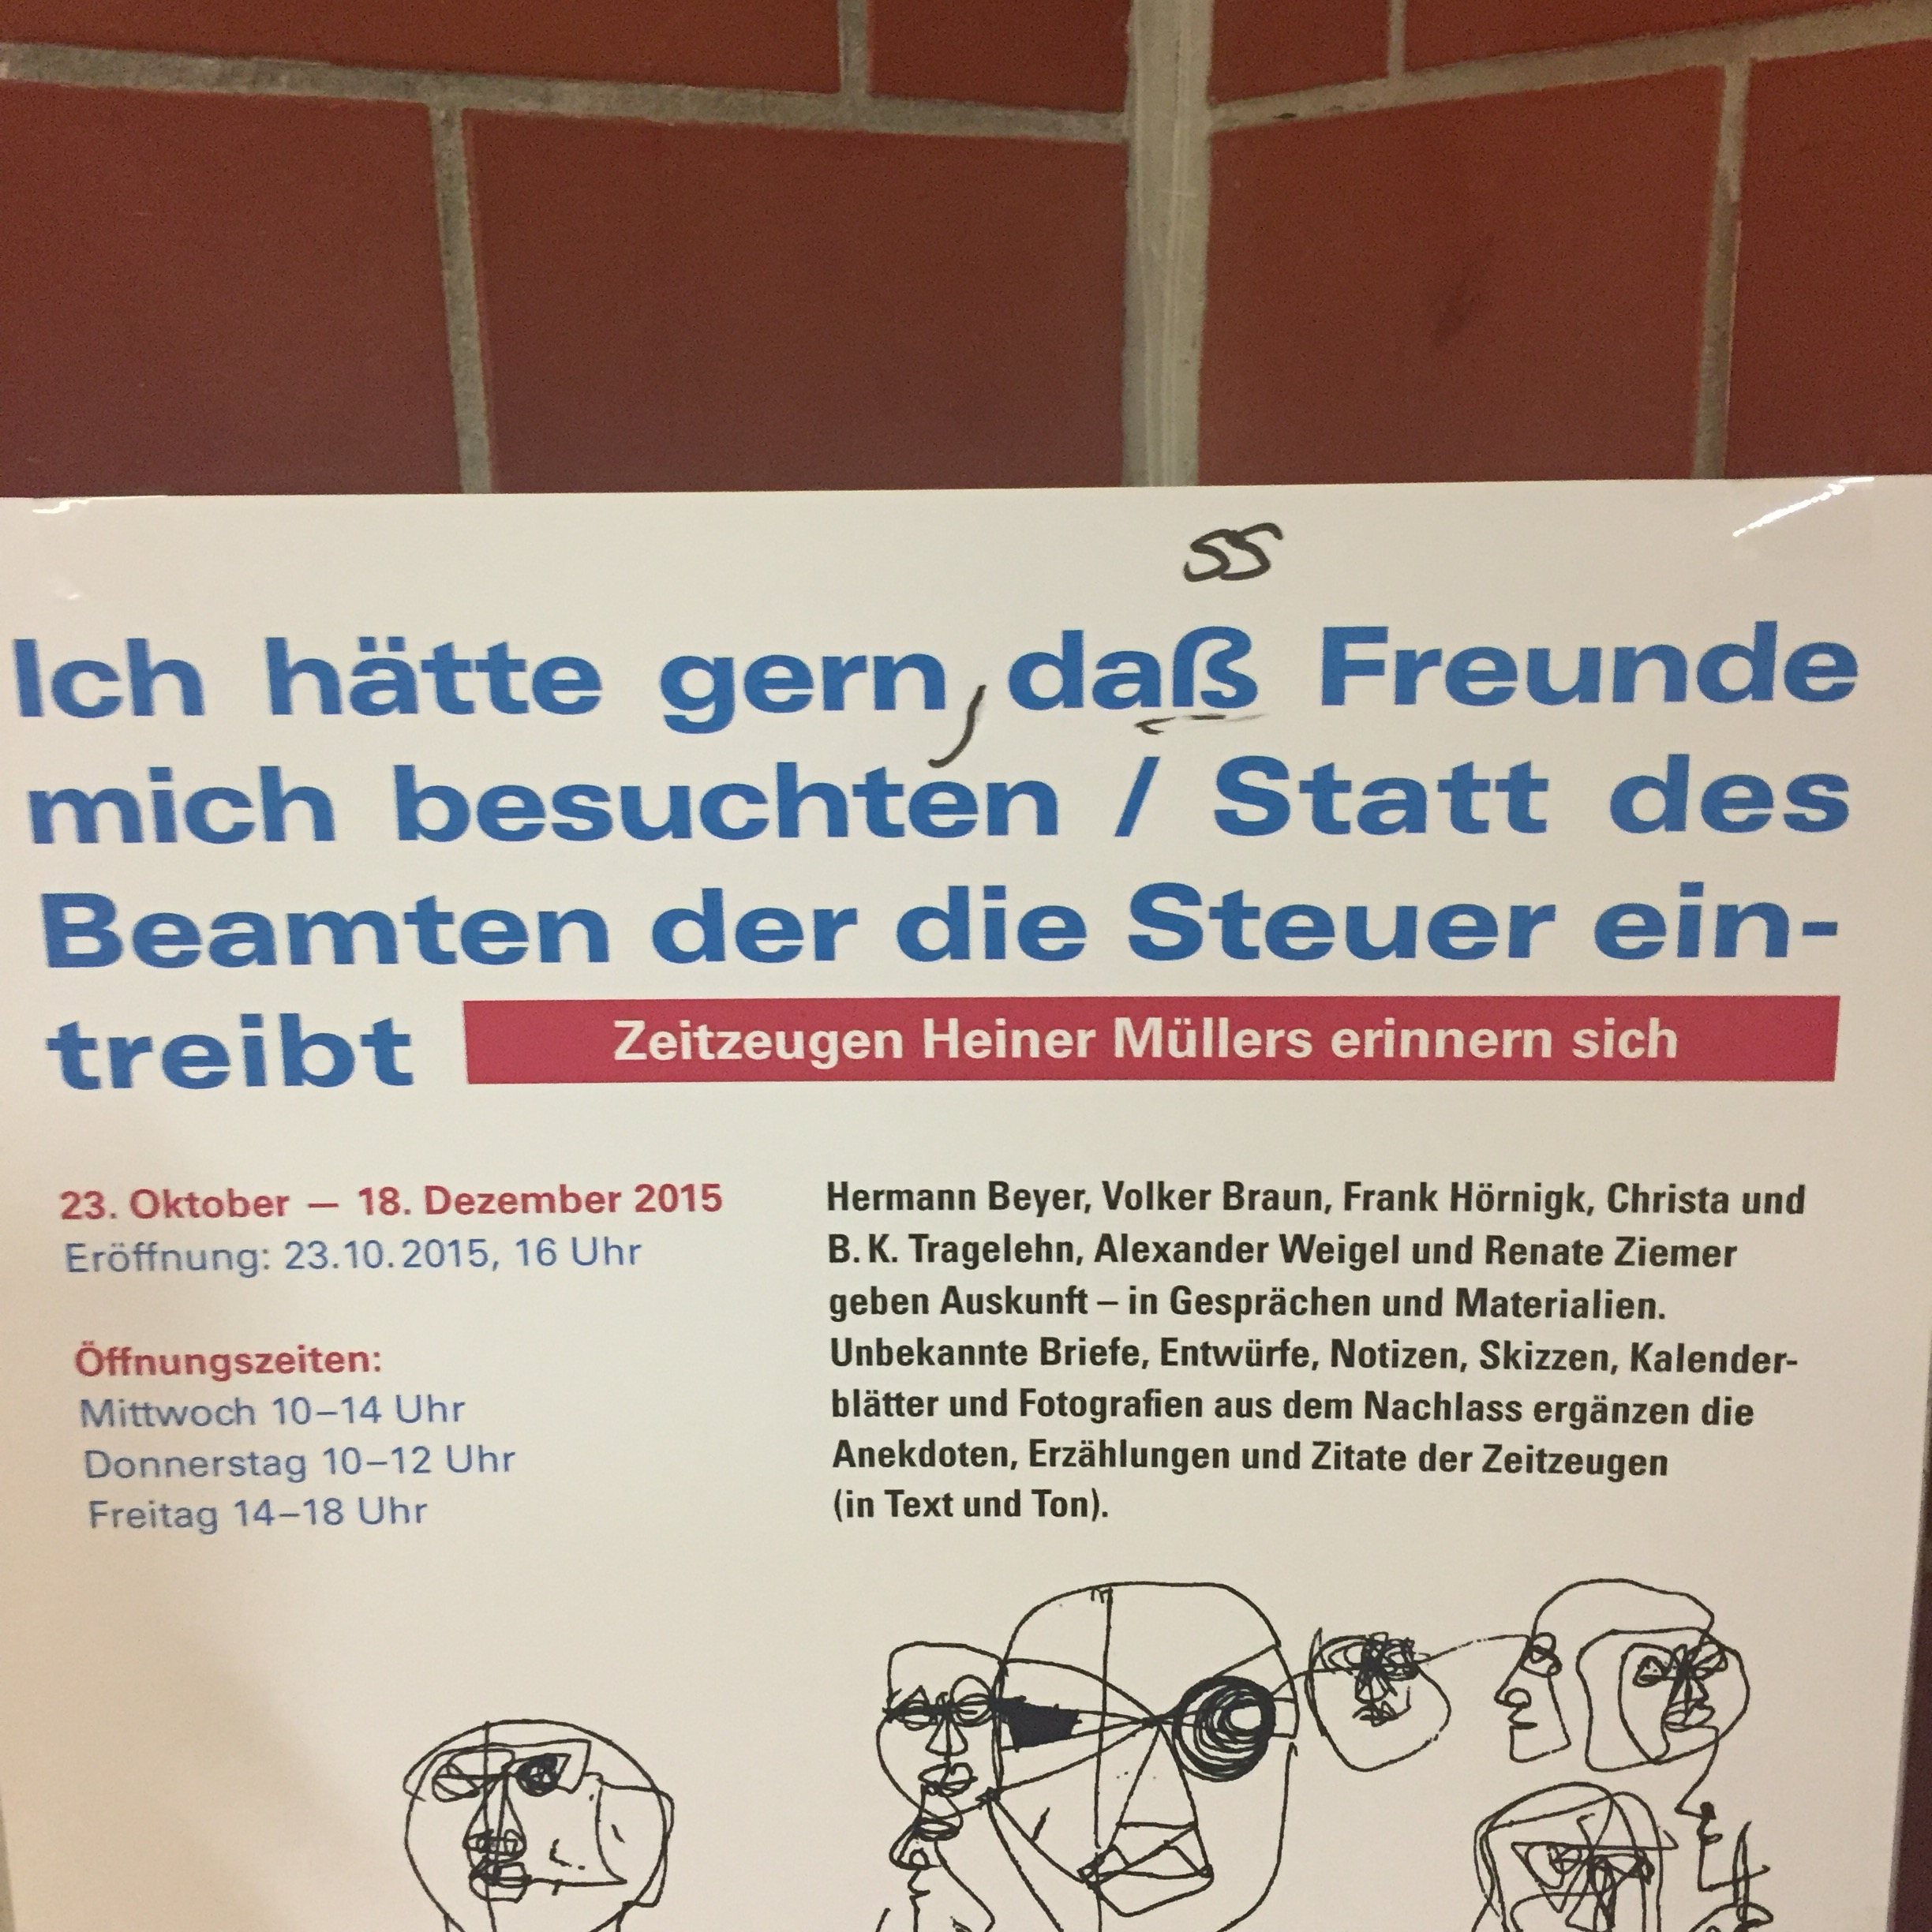
\includegraphics[scale=.065]{material/05praeskriptiv}
%	\caption{Das ist (unangemessen) präskriptiv.}\label{Abb2}
%\end{figure}
%
%\end{frame}


%%%%%%%%%%%%%%%%%%%%%%%%%%%%%%%%%%
\begin{frame}
\frametitle{Deskriptiv \vs Präskriptiv}

\begin{itemize}
	\item Arbeitsweise in der Linguistik \ras \textbf{Deskriptiv} (beschreibend)

	\item Ein Phänomen, das kompetente Sprecher produzieren, wird \textbf{beobachtet und beschrieben}. 	

\end{itemize}
	
	\ea \alertred{Gestern, ich} war im Kino und plötzlich hat es angefangen zu regnen.
	\z
	
	\ea Die theoretische Entwicklung und die praktische Programmierung solcher Betriebssysteme \alertred{hat} sich zu einem neuen Arbeitsgebiet innerhalb der Datenverarbeitung entwickelt. \hfill \citep{Goschler14a}
	\z
	


\end{frame}

%%%%%%%%%%%%%%%%%%%%%%%%%%%%%%%%%%%%%%%%%

%\begin{frame}
%	\frametitle{Deskriptiv \vs Präskriptiv}
	
%\begin{itemize}
%	\item Vorgehensweise von (einigen) Schulgrammatiken und Sprachakademien \ras \textbf{präskriptiv}

%	\item Es wird \textbf{vorgeschrieben}, wie die Strukturen der Sprache gebildet werden \gqq{müssen}.
%	\end{itemize}	
		
%	\ea Es heißt nicht \MyPobj{wegen dem Job}, sondern \MyPobj{wegen des Jobs}.	
%	\z
	
%\end{frame}


%%%%%%%%%%%%%%%%%%%%%%%%%%%%%%%%%%
\begin{frame}
	\frametitle{Deskriptiv \vs Präskriptiv}
\begin{columns}
%%
\begin{column}{.6\textwidth}

\begin{itemize}
	\item Vorgehensweise von (einigen) Schulgrammatiken und Sprachakademien \ras \textbf{präskriptiv}
	
	\medskip
	\item Es wird \textbf{vorgeschrieben}, wie die Strukturen der Sprache gebildet werden \gqq{müssen}.	

\ea Es heißt nicht \MyPobj{wegen dem Job}, sondern \MyPobj{wegen des Jobs}.	
\z

	\item präskriptive Regeln:
	
	\item[] \textbf{Stilistik} (\gqq{schöner} oder \gqq{weniger schön})\\
	oder\\
	
	\item[] Regeln für \gqq{\textbf{gutes/richtiges}} \textbf{Deutsch}
\end{itemize}


\end{column}
%%
\begin{column}{.4\textwidth}

\begin{figure}
	\centering
	
\includegraphics[scale=.045]{material/DudenRichtigesDeutsch}
	\caption{Duden \citep{DudenGramm09d}}\label{Abb3}
\end{figure}

\end{column}

\end{columns}
	
\end{frame}


%%%%%%%%%%%%%%%%%%%%%%%%%%%%%%%%%%
\begin{frame}

\begin{itemize}
%	\item Präskriptive Regeln \\
%	\ras Stilistik (\gqq{schöner} oder \gqq{weniger schön})\\
%	oder\\
%	\ras Regeln für \gqq{gutes/richtiges} Deutsch
%	\item[]
	
	\item In der Linguistik wird auf der Basis von \textbf{deskriptiven Beobachtungen} gearbeitet.
	
	\medskip
	
	\item Kompetente Sprecher verwenden ständig Formulierungen wie \MyPobj{wegen dem Job}, aber nie solche wie:
	
	\ea[*]{Ich bin \alertred{wegen der Job} gekommen.}
%	\z
	
	\ex[*]{Ich bin \alertred{dem wegen Job} gekommen.}
%	\z
	
	\ex[*]{Ich bin \alertred{wegen Job dem} gekommen.}
	\z
	
	\medskip
	\item Diese Formulierungen sind \textbf{ungrammatisch}, denn sie verletzen Regeln des deutschen \textbf{grammatischen Systems}:
	
	\begin{itemize}
		\item Präpositionen stehen \MyPobj{vor} Nominalphrasen
		\item Artikel stehen \MyPobj{vor} dem Nominalkomplex
	\end{itemize}	
	
\end{itemize}

\end{frame}


%%%%%%%%%%%%%%%%%%%%%%%%%%%%%%%%%%
%%%%%%%%%%%%%%%%%%%%%%%%%%%%%%%%%%
\subsection{Abbildungen}


%%%%%%%%%%%%%%%%%%%%%%%%%%%%%%%%%%
\begin{frame}{Abbildungen}
\small

\begin{itemize}
	%\item ABBILDUNG -- \gqq{Glowing blue binary code on screen with word error background concept} (Stock-Foto, Zugriff: 11.05.18)
	%\url{https://www.colourbox.de/bild/bild-26254540}

%	\item ABBILDUNG -- Machicao y Priemer, Antonio: \gqq{Deskriptiv vs. Präskriptiv} (Privatfoto)
	
	\item ABBILDUNG -- Machicao y Priemer, Antonio: \gqq{Duden} (Privatfoto)
\end{itemize}	

\end{frame}

